\chapter{Translations management}

\section{Translation module}
The software \tria is sold with a translation module in certain situation.\\
%Dans certain cas, le logiciel \tria est fourni avec un module de traduction.\\

Warning, it is not possible to use \tria and the translation module in the same time. You have to close the translation module to see the result in \tria.\\
%Attention, il n'est pas possible d'utiliser simultanément le module de traduction et \tria. Vous devez fermer le module de traduction pour voir le résultat dans \tria.\\

This module allow to translate every text which appear in the schemes set : \\
%Ce module permet de traduire les chaînes de caractères qui apparaissent dans un ensemble de schémas. Ces chaînes correspondent aux noms des éléments suivants :\\

\begin{itemize}
\item Actors
%\item Les acteurs
\item Bricks
%\item Les briques
\item Tools
%\item Les moyens
\item Activity %\item Les activités
\item Action times
%\item Les temps d'actions
\item Steps
%\item Les étapes
\item Objectives
%\item Les objectifs
\item Meanings\\
%\item Les moyens\\
\end{itemize}

The translation module works directly with the data file used in \tria. When a translation is associated to a text, it is automatically used in \tria.
%Le module de traduction travaille directement sur le fichier utilisé par \tria. Lorsqu'une traduction est associée à une chaîne de caractère, elle sera utilisée lors de l'utilisation suivante de \tria.

A filter field is avaible in the top of the window. The filter is applied on the translation and the original text.\\
%Un champ de recherche permet de filtrer les entrées affichées dans la fenêtre. La recherche est effectuée sur le terme initial et sa traduction.\\


%Pour utiliser le texte initial au lieu d'une traduction, il suffit d'effacer entièrement le texte de la traduction.\\
It is possible to get statistics about the translation with the button "Translation statistics" on the bottom left of the window.\\


\section{Datapack translation management}
It is possible to export and to import translation of the datapack. Use the corresponding buttons in the bottom of string translator interface \\
%Il possible d'importer et d'exporter une traduction depuis le module de traduction.\\

Warning, the current translation is lost when a new one is imported. Verify if you need to export before import the new one.\\
%Attention, lors d'une importation, la traduction est perdue. Veillez à exporter cette dernière avant si vous voulez la conserver.\\

It is also possible to change the translation from \tria with the option "Change datapack language" in the Edition menu (see picture \ref{menu_edition}). As in String translator module, the current translation will be lost.\\
%Il est aussi possible de changer la traduction depuis le datapack avec l'option "Changer la langue du datapack" dans le menu Edition (voir image \ref{menu_edition}). De même, la traduction actuelle sera écrasée lors de cette opération.\\


\begin{figure}[h!]
\centering
\Ovalbox{
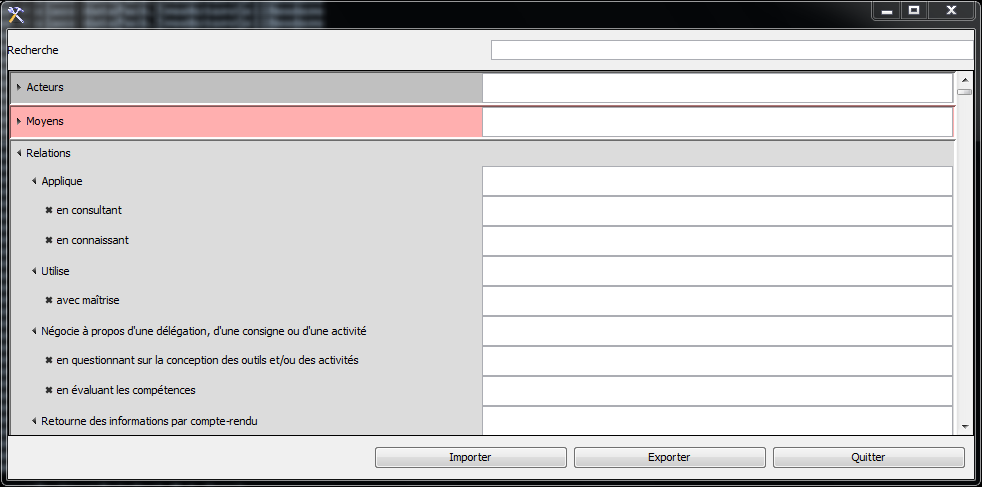
\includegraphics[width=0.8\textwidth]{images/translator.png}
}
\caption{The string translator interface.}
\end{figure}


\section{Selection of software interface language}
The language of software interface can be changed with the "Language" menu in the main window. The software needs to be restarted after a change of language.
%La langue de l'interface peut être choisie à l'aide du menu "Langue" dans l'interface principale. Le logiciel doit être redémarré après un changement de langue.\\

It is possible to add a new language by adding the corresponding file in the sub-folder "language" in the installation \tria folder. To do so, make a copy of any other language file, rename it with the correct code and translates every sentences in the file. The new language will be automatically added to the list of available language in the "Language" menu.\\
%Il est possible d'ajouter une nouvelle langue en ajoutant le fichier correspondant dans le sous dossier "language" du répertoire d'installation du logiciel. Pour réaliser cette traduction, il suffit de réaliser une copie d'un des fichier puis de traduire l'ensemble des phrases qu'il contient. La nouvelle langue sera proposée dans le menu "Langue" lors du démarrage suivant du logiciel.\\

If some sentences are not translated in the software, that could comes from missing sentences in the translation file. In this case, french translation is used instead. That could be corrected by adding the missing sentences in the corresponding file in the language folder.\\
%Si des phrases sont manquantes dans un fichier de traduction, celles de la version françaises seront automatiquement utilisées à la place. De ce fait, si certaines phrases sont en français, cela signifie sûrement que leur traduction est manquante. 


